\chapter{\noun{Communication}}
\begin{figure}[h]
\centering
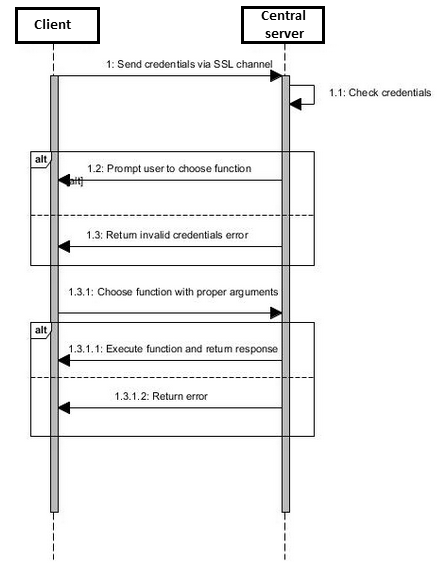
\includegraphics[width=0.7\textwidth]{database/sequence.png}
\caption{General communication diagram for patient, pharmacist and doctor}
\end{figure} 
Every communication with database can be described by one abstract scenario.
First central server and client establish session via SSL. After correct establishment of session, client chooses one of database functions that he can execute with appropriate arguments. Before using methods requiring signatures, client has to ask server for nonce, generated specially for the user. After obtaining the nonce, client can execute selected function.
Database verifies the correctness of signature and data passed in arguments and returns the result, or if one of the verification steps failed, error message.


\section{\noun{Connecting to Central Server}}\label{sec:login}
\begin{enumerate}
\item Enter smartcard with users private key and certificate (or establish paths to them)
\item set path of PostgreSQL to environment variable PATH.

\item in command line write $psql$ $'host=hosts_ip$ $port=port\_address$ $dbname=database\_name$ $user=username$ $sslmode=require$ $sslcert=user.crt$ $sslkey=user.key$ $sslrootcert=ca.crt'$ where:
	\begin{packed_enum}
	\item $host$ - IP of server where database is
	\item $dbname$ - is the name of database to which we want to connect
	\item $user$ - name of user which want to connect. Each part will have its own user name.
	\item $sslcert$ - certificate of user.
	\item $sslkey$ - private key of user.
	\item $sslrootcert$ - Certificate of CA.
	\end{packed_enum}
	Example login: $psql$ $'host=95.85.28.156$ $port=5432$ $dbname=PrescriptionSystemMk2$ $user=patient$ $sslmode=require$ $sslcert=patient.crt$ $sslkey=patient.key$ $sslrootcert=ca.crt'$
\item enter password
\end{enumerate}

\section{\noun{Nonces \& Verification Proccess}}

Randomly generated nonces are part of challenge-response protocol used in communication with database layer. Nonce are security measure against the replay attack. If a request require signature of any party, client has to ask database for generated nonce for given ID. After nonce is return, client has to:
\begin{enumerate}
 \item Conacatenate function name,
 \item function arguments,
 \item nonce.
 \item Calculate SHA-1 sum over the concatenated elements.
 \item Sign the with appropriate key\footnote{Signing method should be equal to invoking openssl command "openssl rsautl sign" with necessary parameters only}.
 \item Add the signature as the corresponding argument in function.
 \item Send the request.
\end{enumerate}

When the server obtains the request:

\begin{enumerate}
\item Takes users key from the database
\item Validates the signature
\item If the signature is validated, constructs SHA-1 sum in the same way as user
\item compares the verified, signed sum with one calculated in previous point
\item Executes the query if the sums are equal
\item Returns the result to the user
\end{enumerate} 

\clearpage
\begin{figure}[h]
\centering
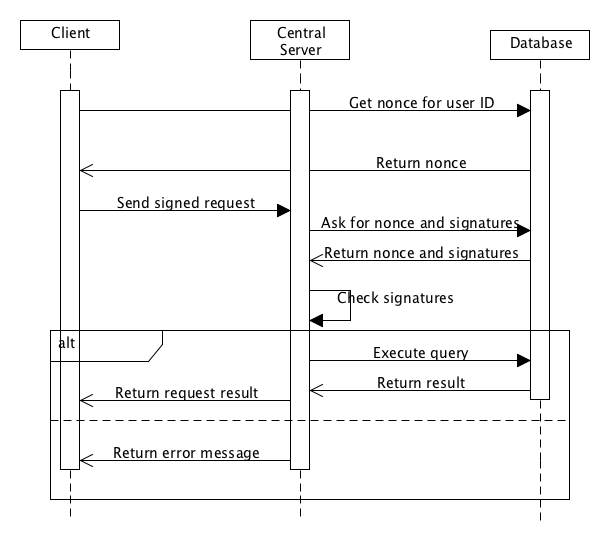
\includegraphics[width=0.8\textwidth]{database/nonce.png}
\caption{Sequence diagram of executing request with nonce signature}
\end{figure} 
